%--------------------------------------------------------------------------------


\documentclass[12pt]{article}
\usepackage[T1]{fontenc}
\usepackage[labelsep=period]{caption}


\usepackage[all]{hypcap}
\usepackage{graphicx}

\usepackage[english]{babel}
\selectlanguage{english}

\usepackage{subfig}
\usepackage{color}
\usepackage{url}

\usepackage{hyperref}
\hypersetup{colorlinks=false, linkbordercolor=1 1 1, citebordercolor=1 1 1}
\usepackage{float}

\usepackage[right]{lineno}
\usepackage{titling}
\renewcommand\linenumberfont{\normalfont\tiny\color{blue}}

\title{\textbf{Computer Vision Course}}

\author{Emanuele Corongiu <xcoron02@stud.fit.vutbr.cz>}
\date{\today}
\maketitle

%--------------------------------------------------------------------------------


\begin{document}
\selectlanguage{english}


\section{introduction and objectives}
In this work, an attempt was made to train a YOLO (You Only Look Once) model for the purpose of recognizing and tracking car license plates. The model was trained under different conditions in order to appreciate some differences in its results.

%%%%%%%%%%%%%%%%%%%%%%%%%%%%%%%%%%%%%%%%%%%%%%%%%%%%%%%%%%%%%%%%%%%%%%%%%%%%%%%%%%%%%%%%

\section{Yolo V8}
Yolo (You Only Lool Once)\cite{yolo1} is a well-known model used for object detection and image segmentation that uses, among other techniques, convolutional neural networks\cite{CV_course_slide}. It represents an excellent tool that is well suited to the purpose of this project, which is given input images, or at least frames of a video, to detect and track license plates of vehicles. Yolo is a powerful and comprehensive tool; the model comes in various sizes and is currently up to version 8 (used here). This tool requires receiving the input dataset by splitting the images into training, validation, and test, respectively, where for each the information within the image should be given in text format. The nano model (3.2M parameters \cite{yolo1}) of YOLO V8 was used in this work.
\clearpage
\section{Dataset}
Two different datasets were used to train the YOLO model in order to observe the difference in the attenuated performance in accordance with the volume of data used. The first step was to train the model with a small dataset\cite{carplate-xuk6s_dataset} containing a total of 301 images. The authors of the dataset obtained, with a yolov8s (11.2M parameters \cite{yolo1}) model, the following results, mAP: 99.5\%, Precision: 97.5\% and Recall: 98.9\%. In the figure \ref{fig:mesh1}, is possible to see more details.

\begin{figure}[H]
    \centering
    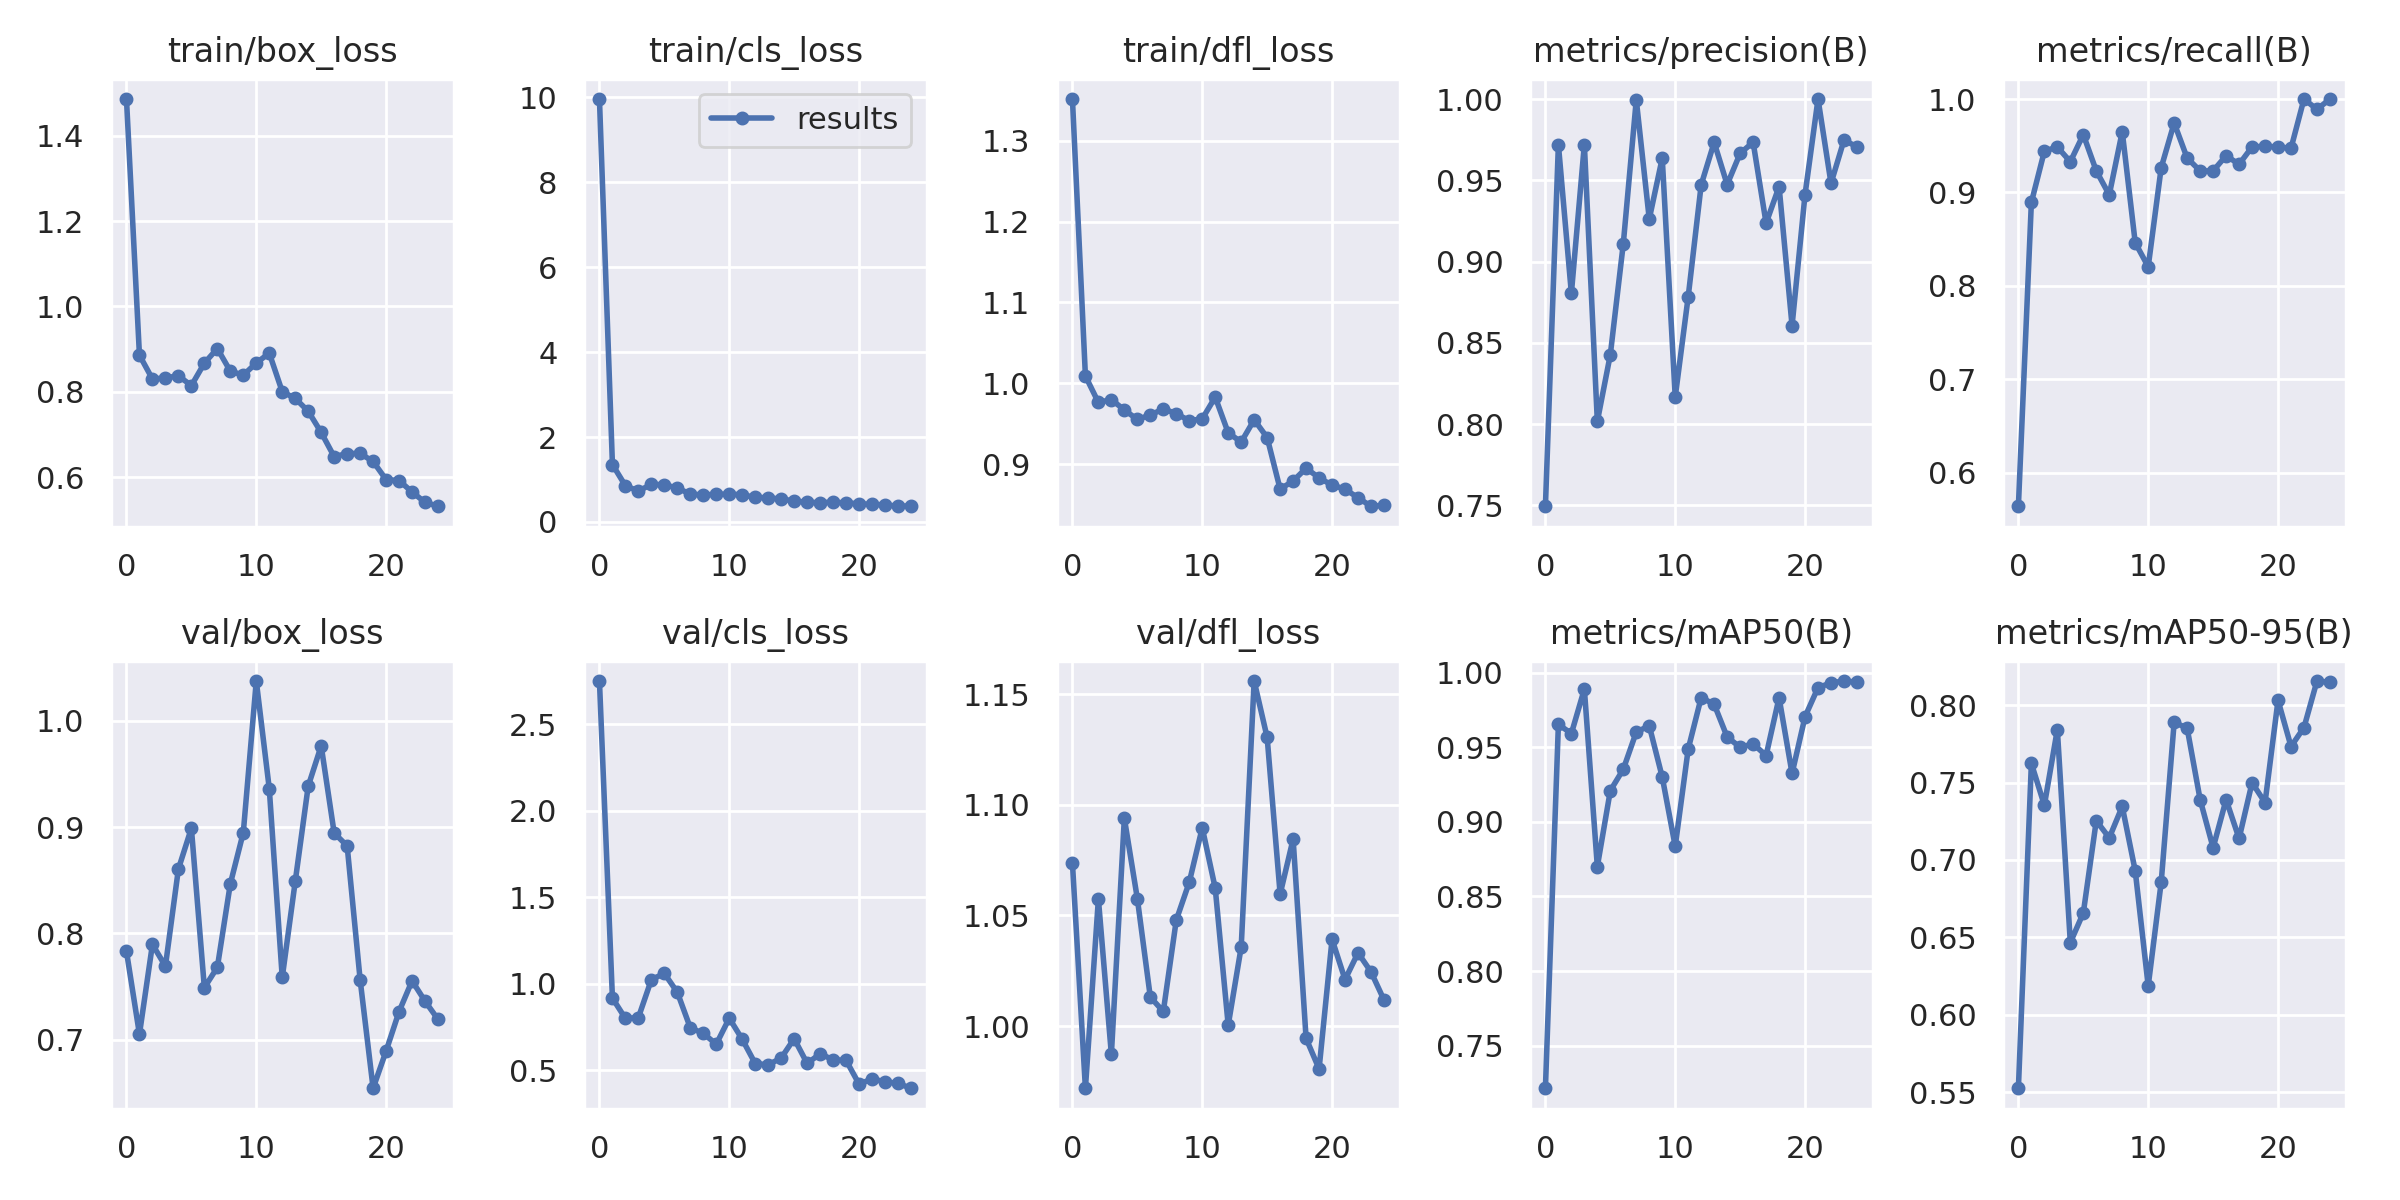
\includegraphics[width=1\linewidth]{results_small dataset.png}
    \caption{Results from \cite{carplate-xuk6s_dataset}}
    \label{fig:mesh1}
\end{figure}

The second dataset\cite{tablice-73he1_dataset} used contained 8683 images of which 6083 were for training, 1733 for validation and 867 for testing.The authors reported the following results with the yolov5 model, mAP: 84.7\%, Precision: 88.8\% and Recall: 80.8\%. In the figure \ref{fig:mesh2}, is possible to see more details.

\begin{figure}[H]
    \centering
    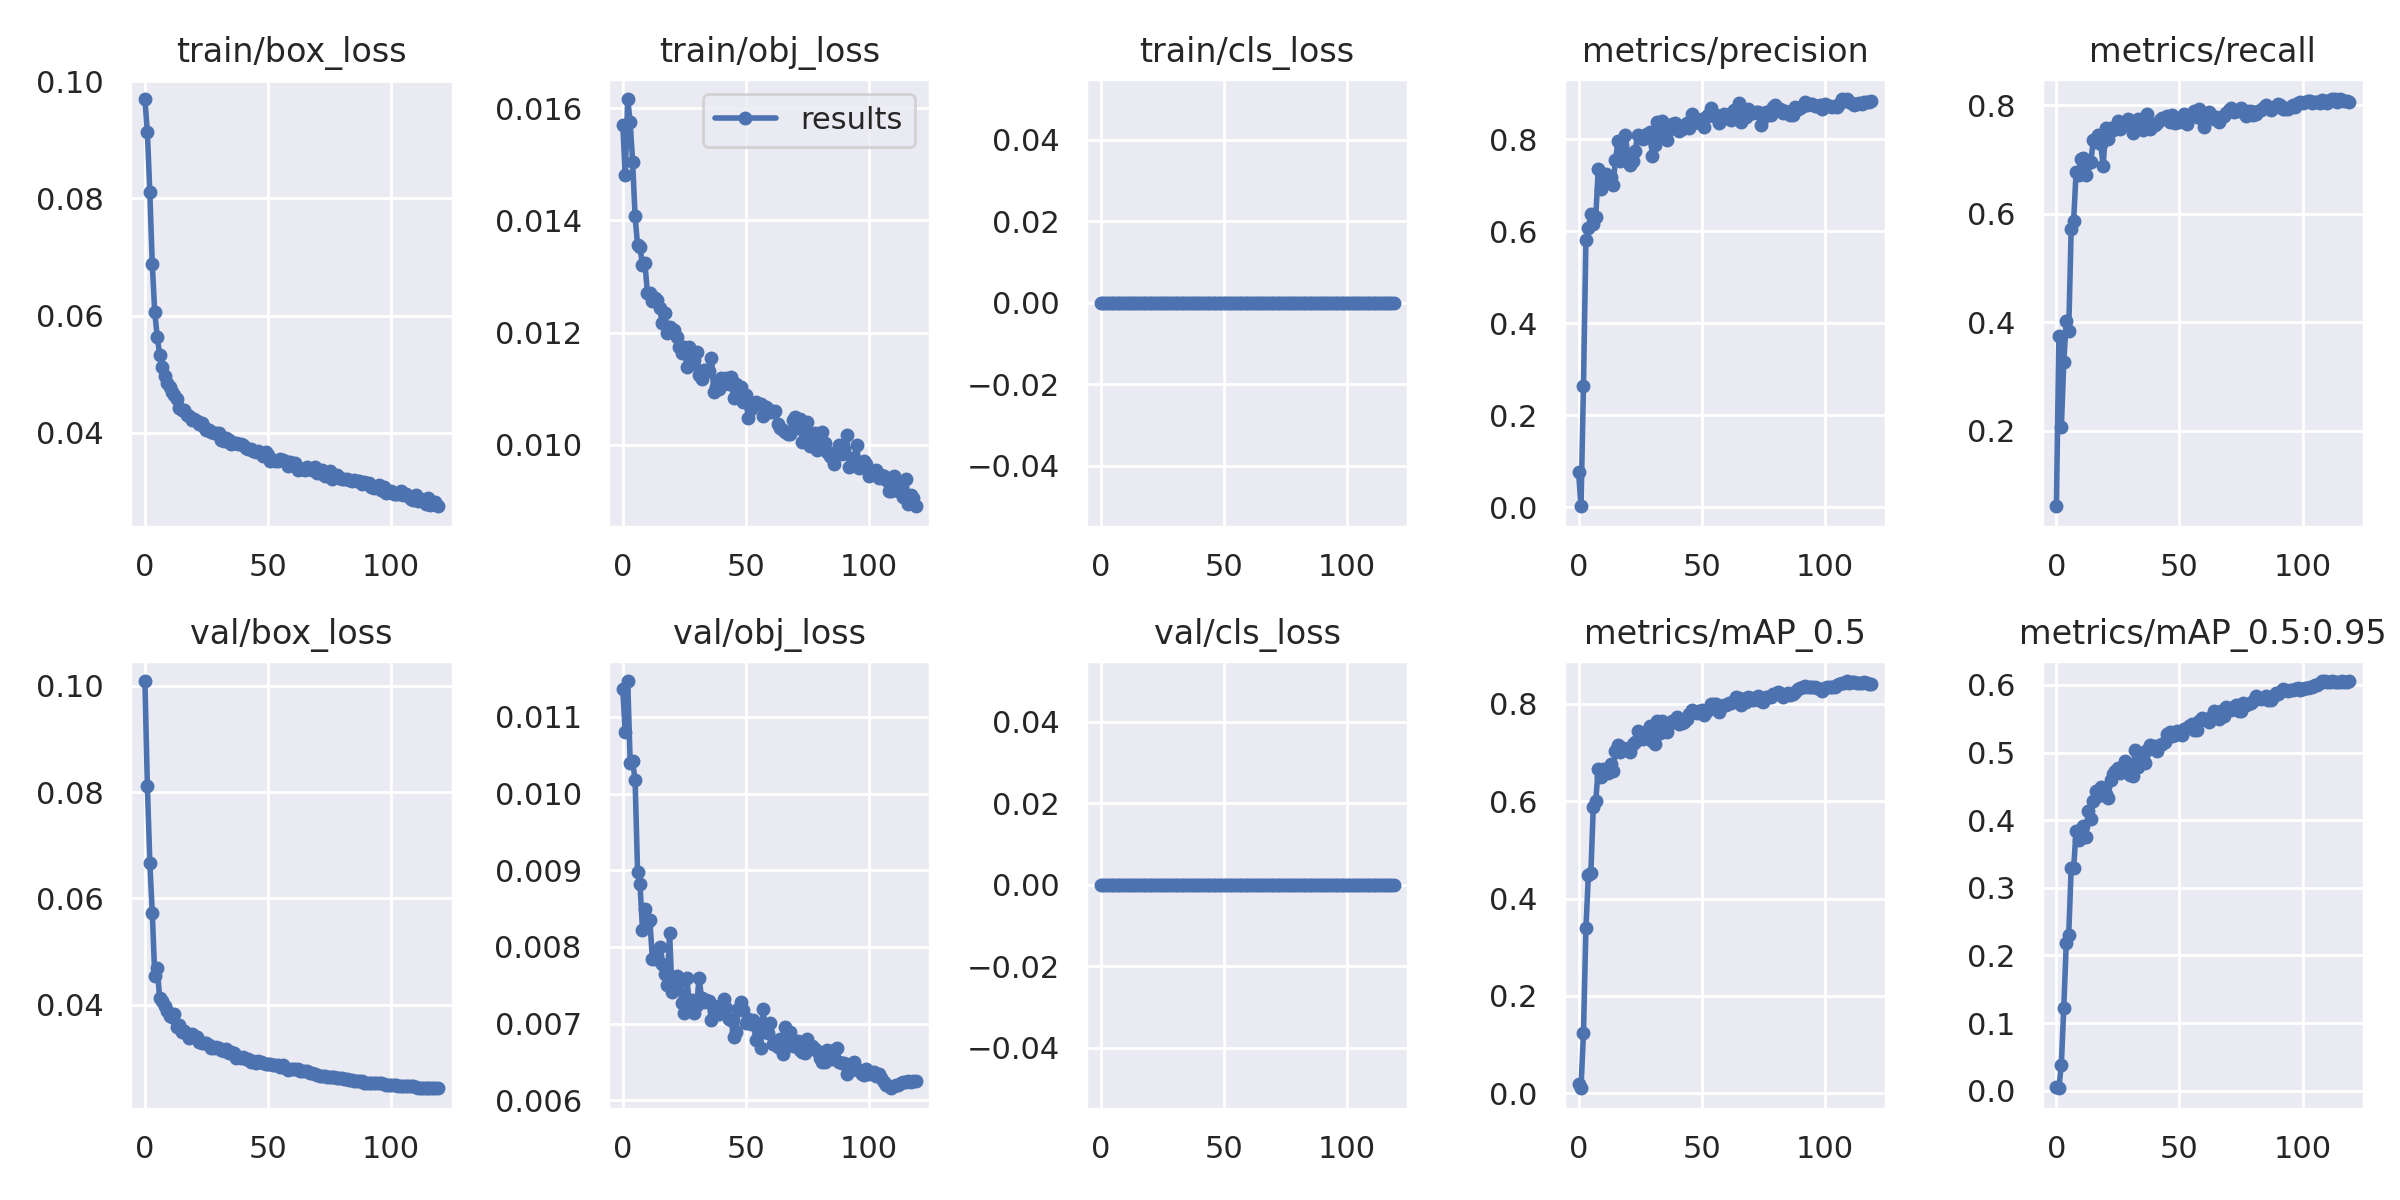
\includegraphics[width=1\linewidth]{results_big_dataset.png}
    \caption{Results from \cite{tablice-73he1_dataset}}
    \label{fig:mesh2}
\end{figure}

\begin{equation}
  \label{moje-rovnice}
  c = a + b
\end{equation}



%%%%%%%%%%%%%%%%%%%%%%%%%%%%%%%%%%%%%%%%%%%%%%%%%%%%%%%%%%%%%%%%%%%%%%%%%%%%%%%%%%%%%%%%



\bibliographystyle{abbrv}
\begin{flushleft}
  \bibliography{main}
\end{flushleft}

%\appendix
%\newpage
%\section{}

\end{document}
